
\title{T-61.5130 Machine Learning and Neural Networks}
\author{Karhunen, Luttinen}
\date{Exercise 10, 7.12.2012}

\usepackage{cancel}

\newcommand{\vect}[1]{{\bf{#1}}}
\newcommand{\svect}[1]{\boldsymbol{#1}}
\newcommand{\matr}[1]{\boldsymbol{#1}}


\begin{document}

\maketitle

\begin{enumerate}


\item Assume a mixture of time-delayed (but not convolved) sources with known delays $D_{ij}$:
  \begin{displaymath}
    x_i(t) = \sum_{j=1}^N a_{ij}s_j(t-D_{ij}),
  \end{displaymath}
  \begin{enumerate}
  \item Show that by Fourier transform, this can be reduced to the instantaneous mixture
    model $\mathbf{X} = \mathbf{A} \mathbf{S}$.
  \item From this mixing matrix $\mathbf{A}$, how do you solve the original mixing
    coefficients $a_{ij}$?
  \end{enumerate}

  \begin{solution}


    \begin{enumerate}
    \item Recall that the Fourier transform of a signal $f(x)$ is
      \begin{align*}
        F(\omega) = \int^{\infty}_{-\infty} f(x) e^{-2\pi i x \omega}
        dx.
      \end{align*}
      We shall use subindices $k$ and $l$ instead of $i$ and $j$ in
      order to avoid confusion with the $i = \sqrt{-1}$.  Denote the
      Fourier transform of the sequence $x_k(t)$ by $X_k(\omega)$ and
      the Fourier transform of $s_l(t)$ by $S_l(\omega)$.  Recall that
      the Fourier transform changes a delay by $D_{kl}$ into
      multiplication with term $e^{i\omega D_{kl}}$.  Fourier
      transforming both sides of the equation defining the mixtures
      thus yields
      \begin{align*}
        X_k(\omega) = \sum_{l=1}^N a_{kl} e^{i\omega
          D_{kl}} S_l(\omega) .
      \end{align*}
      This can be written as $\bf{X}(\omega) = \bf{A}(\omega)
      \bf{S}(\omega)$ when $\bf{X}$ and $\bf{S}$ are defined to be the
      vectors containing $X_k$ and $S_l$ and
      \[
      \bf{A}(\omega) = \left( \begin{array}{ccc} a_{11}e^{i\omega
            D_{11}} & \cdots & a_{1N}e^{i\omega D_{1N}} \\ \vdots & \ddots &
          \vdots \\ a_{M1}e^{i\omega D_{M1}} & \cdots & a_{MN}e^{i\omega
            D_{MN}} \end{array} \right) \, .
      \]
      Notice that ${\bf A}$ is not constant and that the terms
      $e^{i\omega D_{kl}}$ only affect the phase but not the magnitude
      of the components.

    \item Clearly, the original mixing coefficients are obtained from
      $\mathbf{A}(0)$ because $e^{i \cdot 0 \cdot  D_{kl}}=1$.
      % Since the original $a_{kl}$ are real, we have $a_{kl} = \pm
      % |A_{kl}|$, where $A_{kl}$ denotes the element of matrix $\bf{A}$.
    \end{enumerate}
  \end{solution}

  
\item The kurtosis (fourth-order cumulant) of a random variable $x$ is
  defined by
  \begin{displaymath}
    \mathrm{kurt}(x) = E\{(x-E\{x\})^4\}-3(E\{(x-E\{x\})^2\})^2 .
  \end{displaymath}
  By using this definition, prove the following properties of
  kurtosis: If $x_1$ and $x_2$ are independent random variables, then
  %\begin{enumerate}
  %\item 
    \begin{displaymath}
      \mathrm{kurt}(x_1 + x_2) = \mathrm{kurt}(x_1) + \mathrm{kurt}(x_2)
    \end{displaymath}
  %\item 
    \begin{displaymath}
      \mathrm{kurt}(\alpha x_1) = \alpha^4 \mathrm{kurt}(x_1)
    \end{displaymath}
    where $\alpha$ is a scalar.
  %\end{enumerate}
  
  \begin{solution}

    Assume that $x_1$ and $x_2$ are independent random variables.
    Let us prove that $\mathrm{kurt}(x_1+x_2)=\mathrm{kurt}(x_1)+\mathrm{kurt}(x_2)$.
    We may without loss of generality assume that $x_1$ and $x_2$ are zero-mean.
    Then the kurtosis of $x_1+x_2$ is
    \begin{align*}
      \mathrm{kurt}(x_1+x_2) &= E\{(x_1+x_2)^4\}-3(E\{(x_1+x_2)^2\})^2
      \\
      &= E\{x_1^4 + 4 x_1^3 x_2 + 6 x_1^2 x_2^2 + 4 x_1 x_2^3 +
      x_2^4\} -3(E\{x_1^2 + 2 x_1 x_2 + x_2^2\})^2
    \end{align*}
    Expectation is a linear operation, ie. $E\{\alpha y_1+ \beta
    y_2\}=\alpha E\{y_1\}+ \beta E\{y_2\}$ for random variables $y_1$
    and $y_2$ and scalar multipliers $\alpha$ and $\beta$.  The above
    formula can therefore be rewritten as
    \begin{align*}
      &= E\{x_1^4\} + 4 E\{x_1^3 x_2\} + 6 E\{x_1^2 x_2^2\} + 4 E\{x_1
      x_2^3\} + E\{x_2^4\} -3(E\{x_1^2\} + 2 E\{x_1 x_2\} +
      E\{x_2^2\})^2
    \end{align*}
    Since $x_1$ and $x_2$ are independent, $E\{x_1^p x_2^q\} =
    E\{x_1^p\} E\{x_2^q\}$, for all $q,p \in \{1,\ldots,4\}$.  Then
    the above formula can be further rewritten:
    \begin{align*}
      &= E\{x_1^4\} + 4 E\{x_1^3\}\underbrace{E\{x_2\}}_{=0} + 6
      E\{x_1^2\}E\{x_2^2\} + 4 \underbrace{E\{x_1\}}_{=0}E\{x_2^3\} +
      E\{x_2^4\} -3(E\{x_1^2\} + 2
      \underbrace{E\{x_1\}}_{=0}\underbrace{E\{x_2\}}_{=0} +
      E\{x_2^2\})^2
      % \\
      % &= E\{x_1^4\} + 4 E\{x_1^3 x_2\} + 6 E\{x_1^2 x_2^2\} + 4 E\{x_1
      % x_2^3\} + E\{x_2^4\} -3 E\{x_1^2\}^2 -12 E\{x_1^2\} E\{x_1 x_2\}
      % -6 E\{x_1^2\} E\{x_2^2\} -12 E\{x_1 x_2\}^2 -12 E\{x_1 x_2\}
      % E\{x_2^2\} -3 E\{x_2^2\}^2 .
    \end{align*}
    Here, $E\{x_1\}=E\{x_2\}=0$, so the above reduces to
    \begin{align*}
      &= E\{x_1^4\} + 6 E\{x_1^2\}E\{x_2^2\} + E\{x_2^4\}
      -3(E\{x_1^2\} + E\{x_2^2\})^2
      \\
      &= E\{x_1^4\} + \cancel{6 E\{x_1^2\}E\{x_2^2\}} + E\{x_2^4\} -3
      E\{x_1^2\}^2 - \cancel{6 E\{x_1^2\} E\{x_2^2\}} -3 E\{x_2^2\}^2
      \\
      &=E\{x_1^4\} -3 E\{x_1^2\}^2 + E\{x_2^4\} -3 E\{x_2^2\}^2
      \\
      &= \mathrm{kurt}(x_1) + \mathrm{kurt}(x_2) .
    \end{align*}
    
    % \begin{displaymath}
    %   kurt(x_1+x_2)
    %   = E\{x_1^4\} + 4 E\{x_1^3\}E\{x_2\} + 6 E\{x_1^2\}E\{x_2^2\} + 4 E\{x_1\}E\{x_2^3\}
    %   + E\{x_2^4\}
    % \end{displaymath}
    % \begin{displaymath}
    %   -3 E\{x_1^2\}^2 -12 E\{x_1^2\} E\{x_1\}E\{x_2\} -6 E\{x_1^2\} E\{x_2^2\}
    % \end{displaymath}
    % \begin{displaymath}
    %   -12 E\{x_1\}^2 E\{x_2\}^2 -12 E\{x_1\}E\{x_2\} E\{x_2^2\} -3 E\{x_2^2\}^2 .
    % \end{displaymath}
    % Here, $E\{x_1\}=E\{x_2\}=0$, so the above reduces to
    % \begin{displaymath}
    %   kurt(x_1+x_2)
    %   = E\{x_1^4\} + 6 E\{x_1^2\}E\{x_2^2\}
    %   + E\{x_2^4\}
    %   -3 E\{x_1^2\}^2
    %   -6 E\{x_1^2\} E\{x_2^2\}  -3 E\{x_2^2\}^2 .
    % \end{displaymath}
    % The terms $6 E\{x_1^2\}E\{x_2^2\}$ and $-6 E\{x_1^2\}E\{x_2^2\}$ cancel each other.
    % Rearranging terms, we get
    % \begin{displaymath}
    %   kurt(x_1+x_2)
    %   = E\{x_1^4\} -3 E\{x_1^2\}^2 + E\{x_2^4\} -3 E\{x_2^2\}^2
    %   = kurt(x_1) + kurt(x_2) .
    % \end{displaymath}

    Let us prove the second property $\mathrm{kurt}(\alpha x_1) = \alpha^4
    \mathrm{kurt}(x_1)$.  We have
    \begin{align*}
      \mathrm{kurt}(\alpha x_1) &= E\{(\alpha x_1)^4\} - 3(E\{(\alpha
      x_1)^2\})^2
      \\
      &= E\{\alpha^4 x_1^4\} - 3(E\{\alpha^2 x_1^2\})^2
      \\
      &= \alpha^4 E\{x_1^4\} - 3(\alpha^2 E\{x_1^2\})^2
      \\
      &= \alpha^4 E\{x_1^4\} - 3\alpha^4 (E\{x_1^2\})^2
      \\
      &= \alpha^4 (E\{x_1^4\} - 3(E\{x_1^2\})^2)
      \\
      &= \alpha^4 \mathrm{kurt}(x_1).
    \end{align*}
  

  \end{solution}

  
\item Consider a situation in which scalar inputs of a
  one-dimensional SOM are distibuted according to the probability
  distribution function $p(x)$. A stationary state
  of the SOM is reached when the expected changes in the weight
  values become zero:
  \begin{equation*}
    E[h_{j,i(x)}(x-w_j)]=0 \mbox{.}
  \end{equation*}
  Here $h_{j,i(x)}$ is the value of the neighborhood function for neuron $j$ in the neighborhood
  of the winning neuron $i(x)$ for the input vector $x$.
  What are the stationary weight values in the following cases: \begin{enumerate}
  \item $h_{j,i(x)}$ is a constant for all $j$ and $i(x)$, and
  \item $h_{j,i(x)}$ is the Kronecker delta function?
  \end{enumerate}

  \begin{solution}

    \begin{enumerate}
    \item
      \begin{eqnarray*}
        E[\underbrace{h_{j,i(x)}}_{=constant}(x-w_j)]&=&0\\
        \Rightarrow\;E[(x-w_j)]&=&\int_\mathcal{X}(x-w_j)p(x)dx=0\\
        \Rightarrow\;w_j&=&\int_\mathcal{X}xp(x)dx=E[x]
      \end{eqnarray*}
      This means that all the weights converge to the same point.
      Thus, it does not make sense to use this neighborhood function.

    \item
      \begin{eqnarray*}
        E[\underbrace{h_{j,i(x)}}_{=\delta(j,i(x))}(x-w_j)]&=&0\\
        \Rightarrow\;E[(x-w_j)]&=&\int_\mathcal{X}\delta(j,i(x))(x-w_j)p(x)dx=0
      \end{eqnarray*}
      Let $\mathcal{X}=\bigcup_j\mathcal{X}_j$, where $\mathcal{X}_j$ is the part
      of the input space where $w_j$ is the nearest weight. (Voronoi region
      of $w_j$).
      \begin{eqnarray*}
        & &\int_\mathcal{X}\delta(j,i(x))(x-w_j)p(x)dx=0 \\
        &\Rightarrow&\int_{\mathcal{X}_j}(x-w_j)p(x)dx=0\\
        &\Rightarrow&w_j=\frac{\int_{\mathcal{X}_j}xp(x)dx}{\int_{\mathcal{X}_j}p(x)dx}
        = E[x|x \in \mathcal{X}_j]
      \end{eqnarray*}
      $\omega_j$ is the weighted mean of the Voronoi region.  Note
      that this function is not good in practice because only one
      neuron is updated at a time and there is no neighboring neurons,
      thus SOM does not learn the structure.
    \end{enumerate}
  \end{solution}

  
\item It is sometimes said that the SOM algorithm preserves the
  topological relationships that exist in the input space. Strictly
  speaking, this property can be guaranteed only for an input space of
  equal or lower dimensionality than that of the neural
  lattice. Discuss the validity of this statement.

  \begin{solution}


    Consider the ``Peano curve'' shown in Figure \ref{fig:som}. The
    self-organizing map has a one-dimensional lattice that is taught
    with two-dimensional data. We can see that the data points inside
    the circle map to either unit A or unit B on the map. Some of the
    data points are mapped very far from each other on the lattice of
    the SOM even though they are close by in the input space. Thus the
    topological relationships are not preserved by the SOM. This is
    true in general for any method that reduces dimensionality. It is
    not possible to preserve all the relationships in the data.

    \begin{figure}[h]
      \centering %
      \subfloat[][Random
      initialization]{ 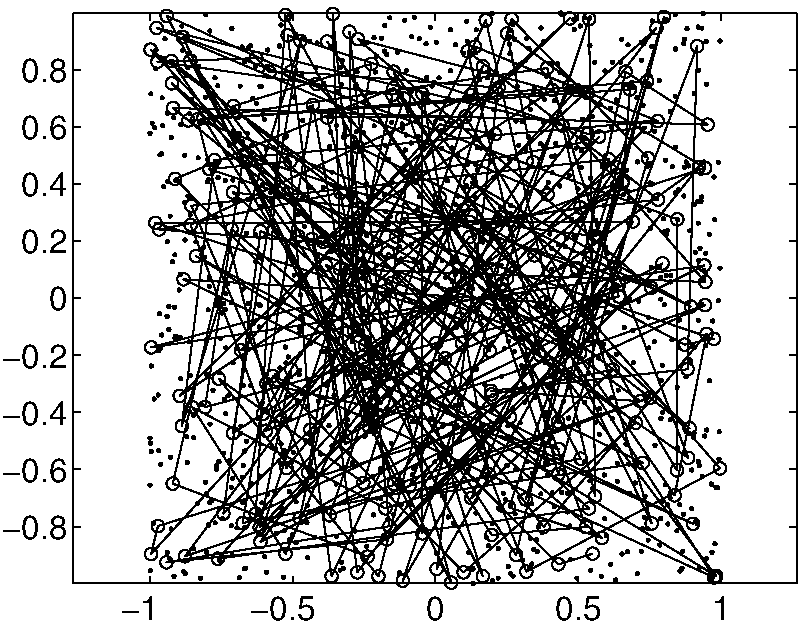
\includegraphics[width=0.45\textwidth]{v121-f1}
      } %
      \hfill %
      \subfloat[][After the ordering
      phase]{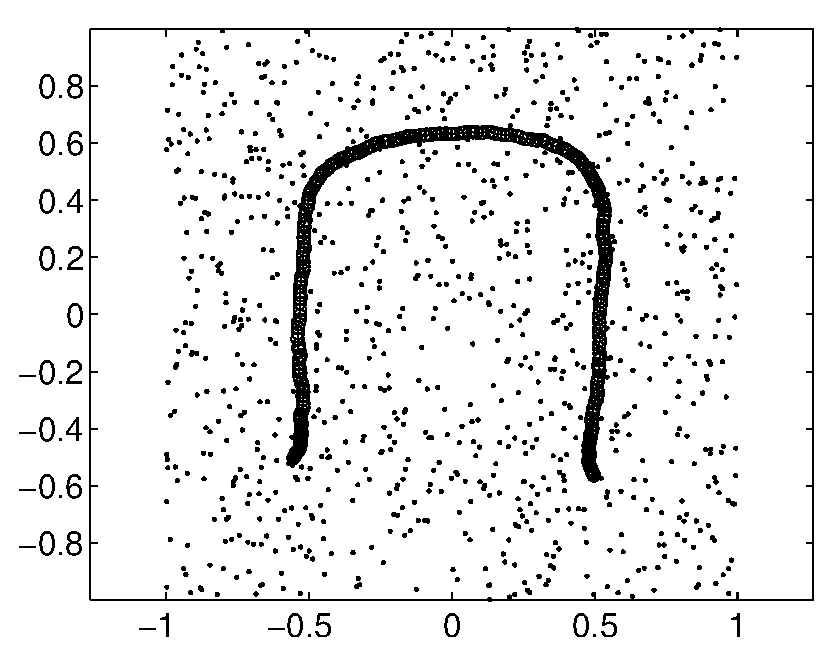
\includegraphics[width=0.45\textwidth]{v121-f2}} %
      \\
      \subfloat[][End of the convergence
      phase\label{fig:som}]{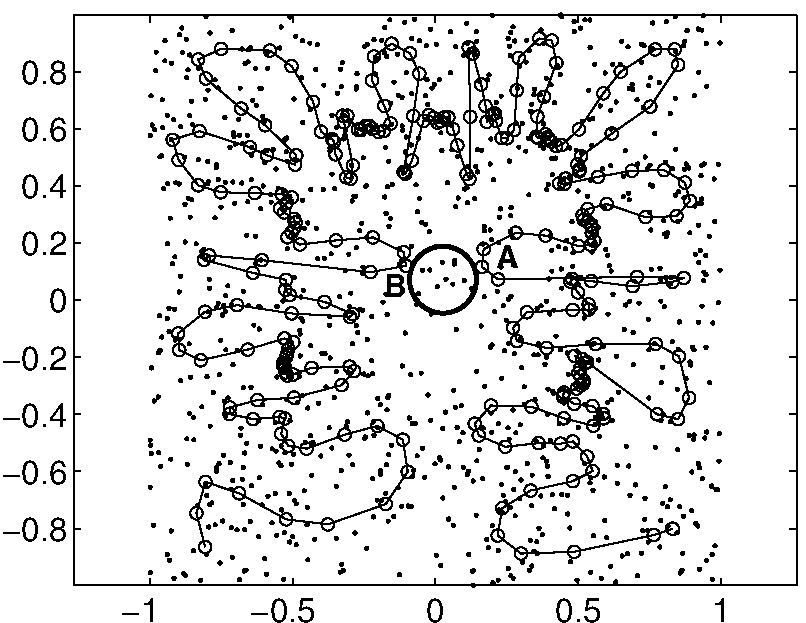
\includegraphics[width=0.45\textwidth]{v121-f3f}}
      \caption{An example of a one-dimensinal SOM with two-dimensional
        input data.  In (c), the circle marks one area where the SOM
        mapping violates the topology of the input space.}
    \end{figure}


  \end{solution}

\item (demo) SOM demo.

  \begin{solution}
    \begin{figure}[h]
      \centering
      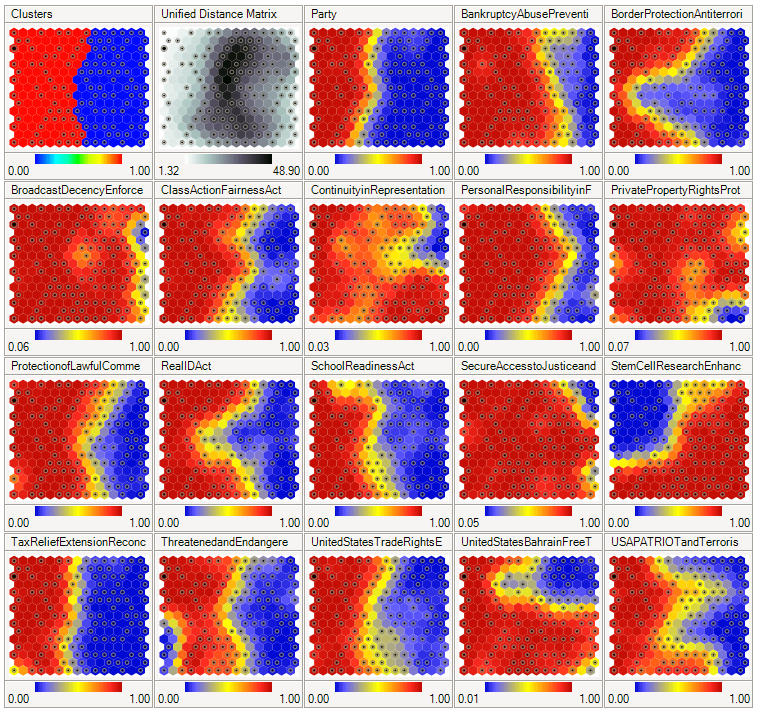
\includegraphics[width=0.8\textwidth]{som_demo.png}
      \caption{SOM showing U.S. Congress voting patterns. The first
        two boxes show clustering and distances while the remaining
        ones show the component planes. Red means a yes vote while
        blue means a no vote in the component planes (except the party
        component where red is Republican and blue is
        Democratic). {\scriptsize Source: Wikipedia. License:
          CC-BY-SA-2.5.}}
    \end{figure}
  \end{solution}

\end{enumerate}
\end{document}             % End of document.

%%% Local Variables: 
%%% mode: latex
%%% TeX-master: "ex10_solutions"
%%% End: 
